\section{OLAP analiza}

Nakon uspješne implementacije ETL procesa i popunjavanja skladišta podataka, konačni korak predstavlja izvršavanje OLAP (Online Analytical Processing) analiza koje omogućuju dubinsko razumijevanje poslovnih trendova i donošenje informiranih odluka. OLAP sustavi omogućuju brze, interaktivne analize velikih količina podataka kroz višedimenzijski pristup \cite{Matosic2015}.

\subsection{Osnove OLAP tehnologija}

OLAP predstavlja kategoriju softverskih alata optimiziranih za analizu i izvještavanje nad skladištima podataka. Za razliku od OLTP (Online Transaction Processing) sustava koji su optimizirani za transakcijske operacije, OLAP sustavi su dizajnirani za analitičke upite koji često zahtijevaju agregirane podatke kroz više dimenzija \cite{Chaudhuri1997}.

Ključne karakteristike OLAP sustava uključuju:

\textbf{Višedimenzijski pristup:}
\begin{itemize}
    \item Podatci se organiziraju u kocke (cubes) s više dimenzija
    \item Omogućuju slice, dice, drill-down i roll-up operacije
    \item Intuitivna navigacija kroz hijerarhije podataka
\end{itemize}

\textbf{Interaktivnost i brzina:}
\begin{itemize}
    \item Sub-sekundni odgovor na kompleksne upite
    \item Mogućnost dinamičkog mijenjanja perspektive analize
    \item Real-time istraživanje podataka
\end{itemize}

\textbf{Složene kalkulacije:}
\begin{itemize}
    \item Podrška za složene poslovne upite i kalkulacije
    \item Vremensko modeliranje i trend analiza
    \item What-if scenariji i prediktivne analize
\end{itemize}

\subsection{Tableau kao OLAP alat}

Za potrebe ovog projekta odabran je Tableau kao vodeći alat za poslovnu inteligenciju koji omogućuje korištenje OLAP funkcionalnosti kroz intuitivno sučelje za vizualizaciju podataka \cite{Murray2013}. Tableau se izravno povezuje na naše MySQL skladište podataka i omogućuje explorativnu analizu po jednostavnom drag-and-drop principu.

Prednosti Tableau-a za OLAP analize:
\begin{itemize}
    \item \textbf{Izravna povezanost} s MySQL skladištem podataka
    \item \textbf{Automatsko prepoznavanje} hierarchija i veza
    \item \textbf{Interaktivne vizualizacije} s drill-down mogućnostima
    \item \textbf{Real-time analiza} bez potrebe za predkompajliranim kockama
\end{itemize}

\subsection{Analiza cijena kroz dimenzije}

Prva skupina analiza fokusira se na ponašanje cijena automobila kroz različite dimenzije, omogućujući identifikaciju ključnih čimbenika koji utječu na vrednovanje vozila.

\subsubsection{Regionalna analiza cijena}

Analiza prosječnih cijena po regijama i desetljećima otkriva značajne geografske i vremenske trendove na automobilskom tržištu.

\begin{figure}[H]
    \centering
    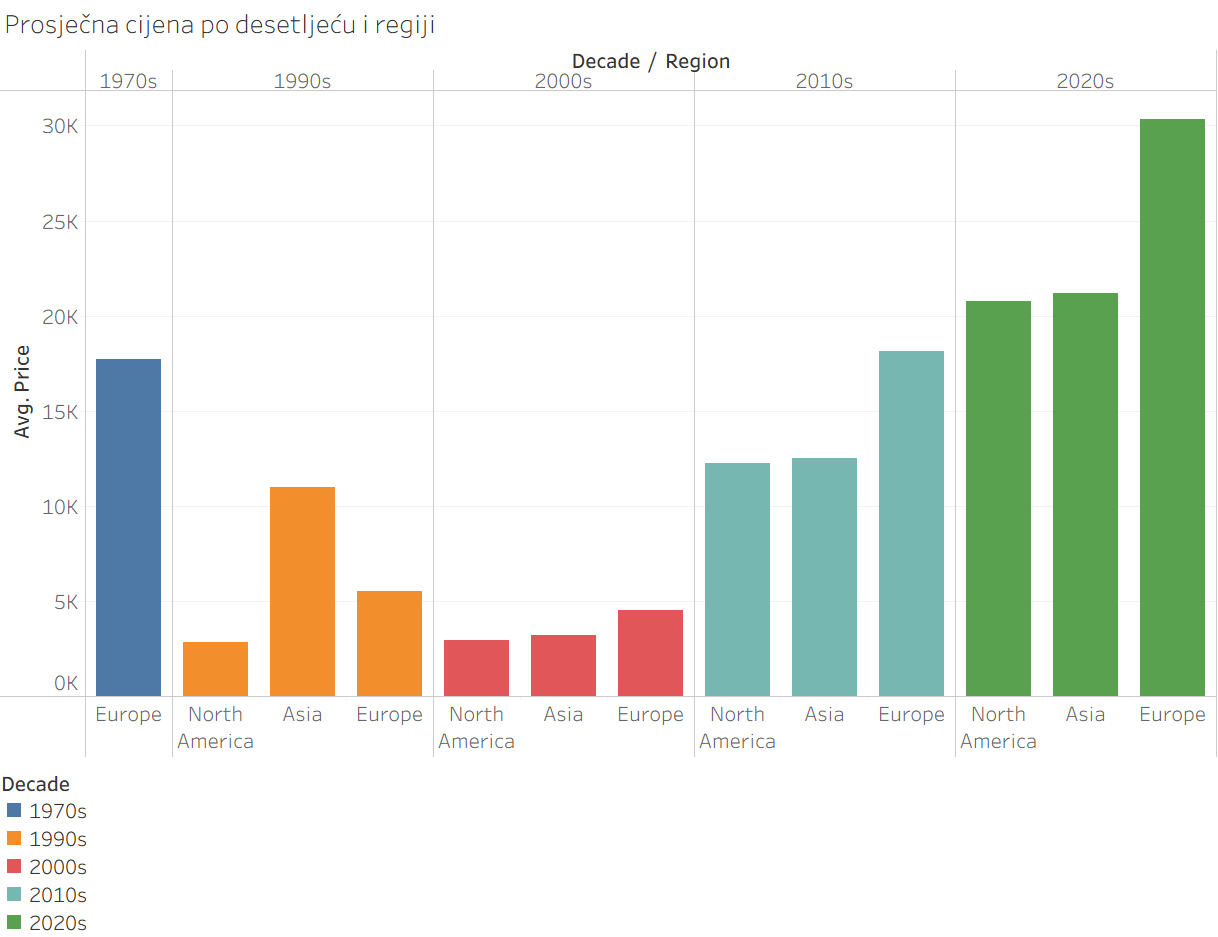
\includegraphics[width=0.9\textwidth]{slike/olap_analiza/1-prosječna-cijena-po-desetljeću-i-regiji.png}
    \caption{Prosječna cijena automobila po desetljeću i regiji}
    \label{fig:cijena-po-regiji-desetljecu}
\end{figure}

Vizualizacija otkriva jasne regionalne i vremenske trendove na automobilskom tržištu. Europski proizvođači konzistentno postižu najviše prosječne cijene kroz sva desetljeća (od 17.747€ u 1970-ima do 30.349€ u 2020-ima), što potvrđuje njihovo pozicioniranje u premium segmentu. Azijski proizvođači zauzimaju srednji cjenovni segment s rastućim trendom od 1990-ih (10.993€) do 2020-ih (21.209€), dok sjevernoamerički proizvođači pokazuju najniže prosječne cijene kroz većinu razdoblja, s izuzetkom značajnog rasta u 2020-ima (20.767€). Ova analiza predstavlja klasičnu OLAP operaciju roll-up po vremenskoj i geografskoj hijerarhiji.

\subsubsection{Analiza po zemljama proizvođača}

Dublja analiza po zemljama proizvođača omogućuje preciznije razumijevanje konkurentnosti na globalnom tržištu.

\begin{figure}[H]
    \centering
    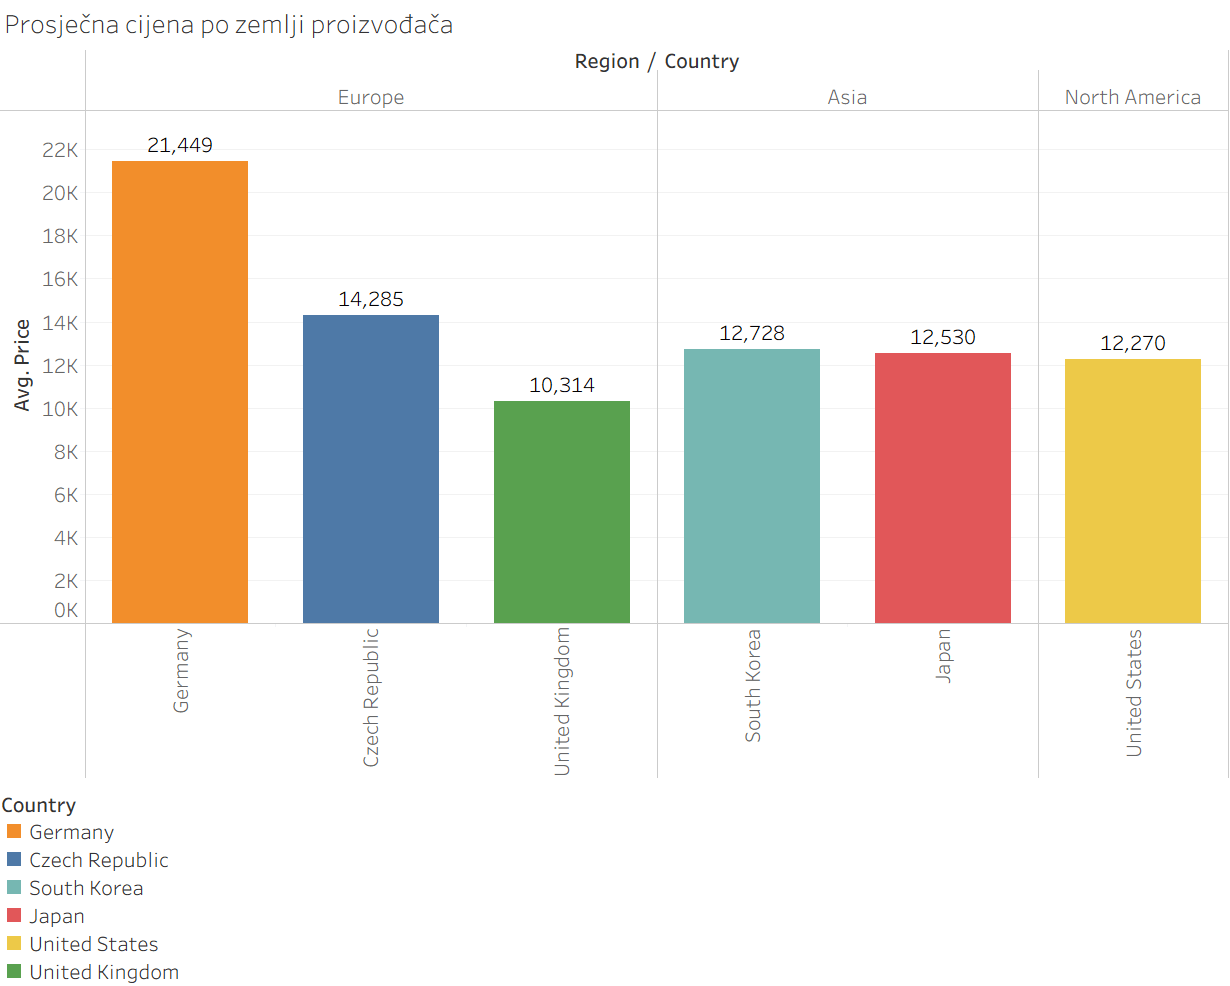
\includegraphics[width=0.9\textwidth]{slike/olap_analiza/2-prosječna-cijena-po-zemlji-proizvođača.png}
    \caption{Prosječna cijena automobila po zemlji proizvođača}
    \label{fig:cijena-po-zemlji}
\end{figure}

Rezultati pokazuju da njemački proizvođači održavaju najviše prosječne cijene, što odražava pozicioniranje na premium tržištu, dok korejski, japanski i američki proizvođači nude kompetitivne cijene u masovnom tržišnom segmentu. Automobili britanskih proizvođača generalno su pristupačniji i povoljniji široj publici.

\subsubsection{Vremenska analiza cijena}

Longitudinalna analiza kretanja cijena kroz vremenski period omogućuje dublje razumijevanje tržišne dinamike i procesa gubitka vrijednosti vozila.

\begin{figure}[H]
    \centering
    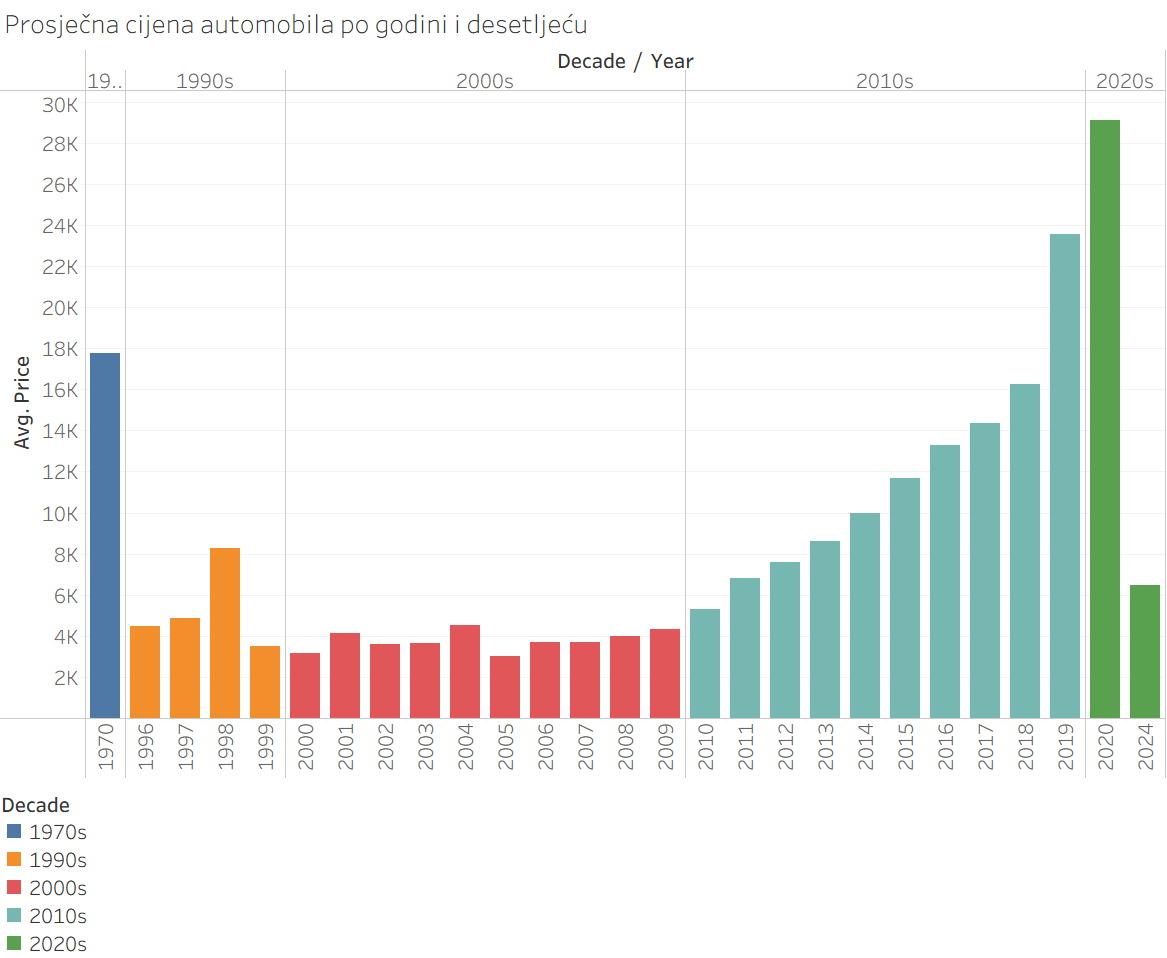
\includegraphics[width=0.9\textwidth]{slike/olap_analiza/3-prosječna-cijena-automobila-po-godini-i-desetljeću.png}
    \caption{Prosječna cijena automobila po godini i desetljeću}
    \label{fig:cijena-po-godini}
\end{figure}

Vizualizacija prikazuje značajne fluktuacije tržišnih cijena kroz različita desetljeća. Najviše prosječne cijene zabilježene su u 1970-ima (oldtimeri) (17.747€) i 2020-ima (29.108€ u 2020.), dok su najniže cijene karakteristične za 2000-e godine (3.017-4.524€). Posebno je uočljiv exponencijalni rast cijena kroz 2010-e godine, od 5.286€ u 2010. do 23.570€ u 2019., što odražava tehnološki napredak, premiumizaciju tržišta i inflacijske pritiske na automobilsku industriju.

\subsection{Analiza proizvođača i modela}

Druga skupina analiza istražuje performanse proizvođača i specifičnih modela, omogućujući rangiranje prema različitim kriterijima.

\subsubsection{Top modeli po cijeni}

Identifikacija najskupljih modela pruža uvid u luksuzni segment tržišta.

\begin{figure}[H]
    \centering
    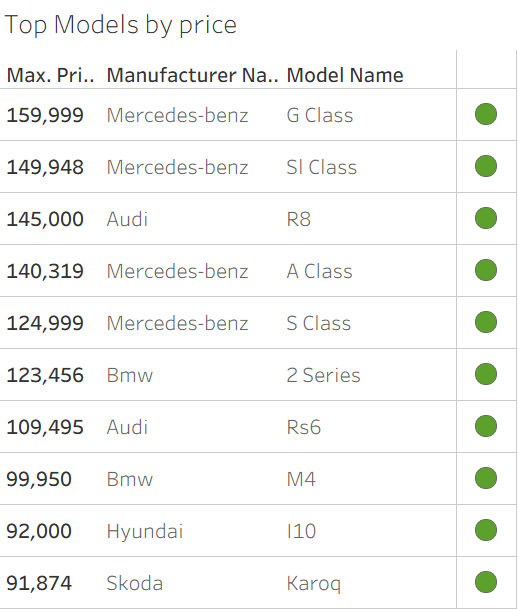
\includegraphics[width=0.9\textwidth]{slike/olap_analiza/5-top-models-by-price.png}
    \caption{Top modeli automobila prema cijeni}
    \label{fig:top-modeli}
\end{figure}

Analiza otkriva dominaciju njemačkih premium proizvođača u vrhu cjenovne hijerarhije, s Mercedes-Benzom koji drži četiri od deset najskupljih pozicija (G Class 159.999€, SL Class 149.948€, A Class 140.319€, S Class 124.999€). BMW i Audi također snažno su zastupljeni s modelima poput BMW 2 Series (123.456€), BMW M4 (99.950€) i Audi R8 (145.000€), Audi RS6 (109.495€). Zanimljivo je prisustvo Hyundai I10 (92.000€) i Škoda Karoq (91.874€) među top modelima, što ukazuje na probijanje tradicionalno mass-market brandova u luksuzni segment.

\subsubsection{Odnos cijene i veličine motora}

Scatter plot analiza otkriva korelaciju između tehničkih specifikacija i cijene.

\begin{figure}[H]
    \centering
    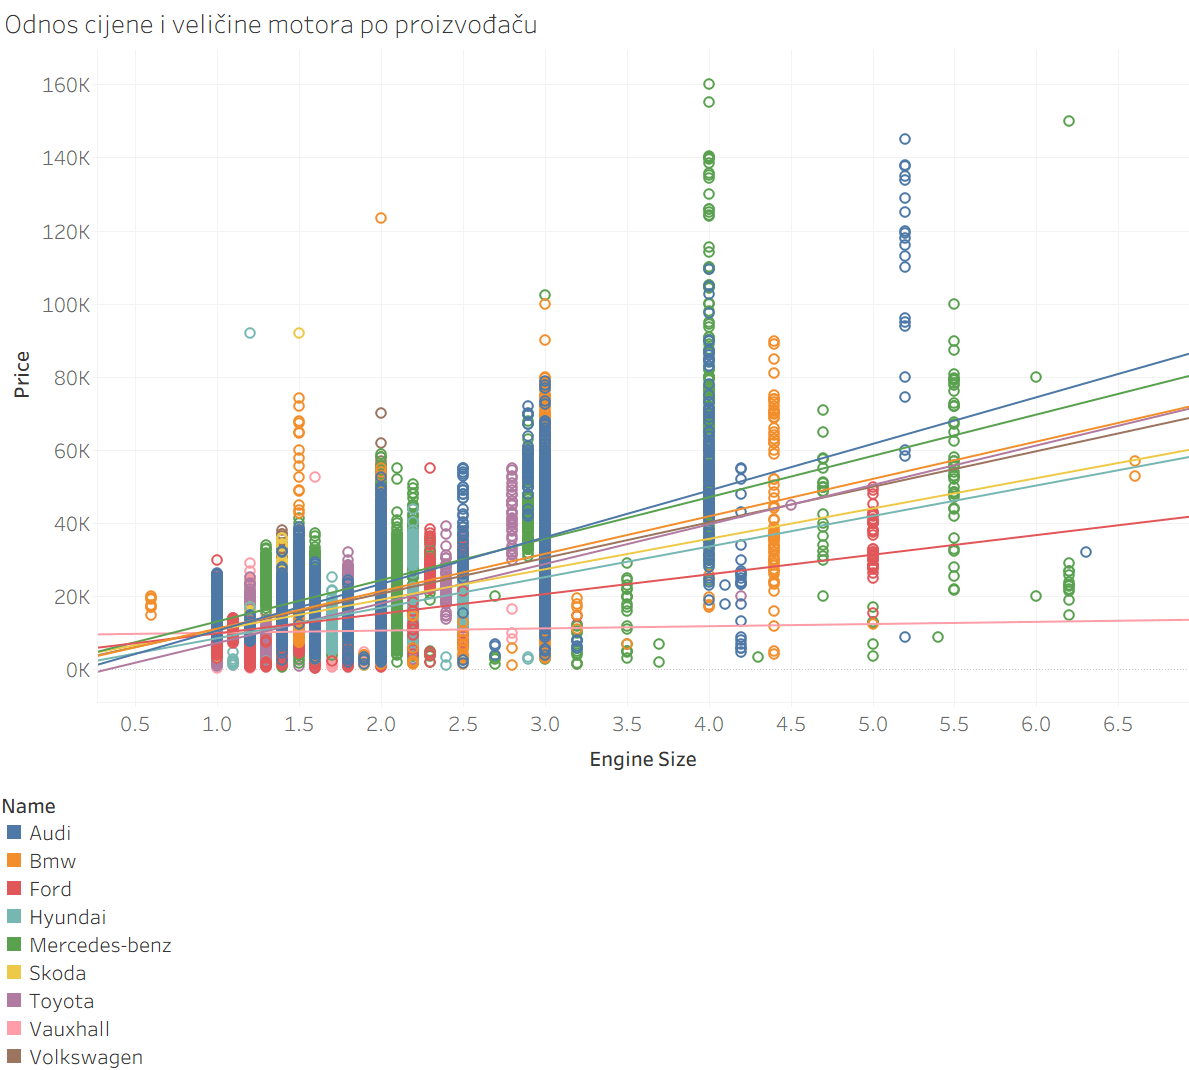
\includegraphics[width=0.9\textwidth]{slike/olap_analiza/6-odnos-cijene-i-veličine-motora-po-proizvođaču.png}
    \caption{Odnos cijene i veličine motora po proizvođaču}
    \label{fig:cijena-velicina-motora}
\end{figure}

Scatter plot analiza jasno potvrđuje snažnu pozitivnu korelaciju između veličine motora i cijene vozila, pri čemu svaki proizvođač demonstrira distinktivnu strategiju pozicioniranja. Audi (plava linija) pokazuje najstrmiji gradijent rasta cijene s veličinom motora, što odražava agresivno premium pozicioniranje s izrazitim fokusom na performanse većih motora. Mercedes-Benz (zelena) također pokazuje snažan trend rasta, ali s nešto umjerenijim nagibom, dok BMW (narančasta) i Volkswagen (ljubičasta) pokazuju umjerene ali konzistentne trendove. Azijski proizvođači Toyota (ružičasta) i Hyundai (tirkizna) uglavnom se pozicioniraju u nižim cjenovnim segmentima neovisno o veličini motora, što ukazuje na strategiju value-for-money. Škoda (žuta) i Ford (crvena) zauzimaju srednji segment s predvidljivim linearnim trendovima, što potvrđuje različite poslovne strategije od mass-market pristupa do premium pozicioniranja.

\subsubsection{Analiza po tipu motora}

Heat mapa pokazuje prosječne cijene prema proizvođačima i tipovima motora.

\begin{figure}[H]
    \centering
    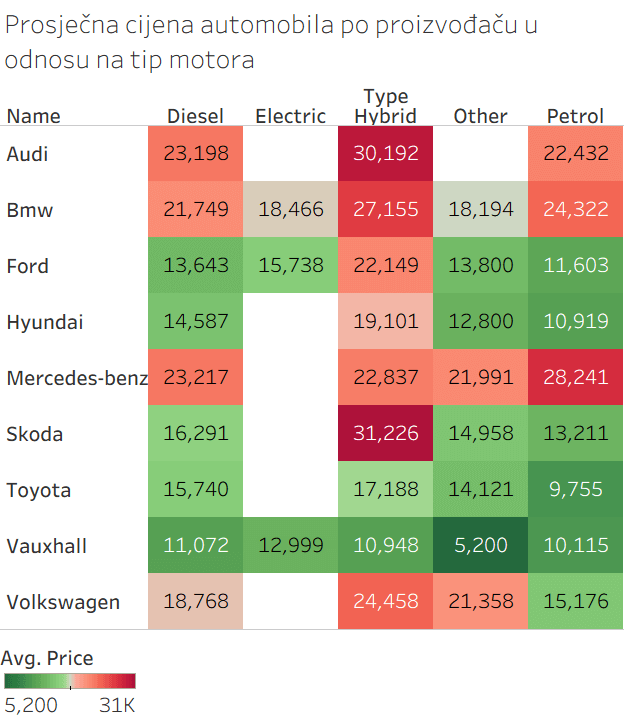
\includegraphics[width=0.9\textwidth]{slike/olap_analiza/7-prosječna-cijena-automobila-po-proizvođaču-u-odnosu-na-tip-motora.png}
    \caption{Prosječna cijena automobila po proizvođaču u odnosu na tip motora}
    \label{fig:cijena-tip-motora}
\end{figure}

Heat mapa analiza otkriva jasne cjenovne razlike između tipova motora kroz sve proizvođače. Hibridni motori dominiraju u cijeni s prosječnim cijenama od 10.948€ (Vauxhall) do 31.225€ (Škoda), pri čemu premium brandovi BMW (27.154€) i Audi (30.191€) pozicioniraju hibride u luksuzni segment. Električni motori, iako ograničeno zastupljeni, pokazuju umjerene cijene (BMW 18.466€, Ford 15.737€, Vauxhall 12.999€). Dizelski motori zauzimaju srednji cjenovni segment s rasponom od 11.071€ (Vauxhall) do 23.216€ (Mercedes-Benz), dok benzinski motori pokazuju najširi spektar cijena od 9.754€ (Toyota) do 28.240€ (Mercedes-Benz), potvrđujući njihovu dominaciju kroz sve tržišne segmente. Kategorija "Other" (uključujući LPG i CNG) generalno se pozicionira između benzinskih i dizelskih motora po cijeni.

\subsubsection{Detaljna analiza po modelu}

Stupčasti dijagram pruža pregled prosječnih cijena po proizvođačima i modelima, rangirajući ih po vrijednosti.

\begin{figure}[H]
    \centering
    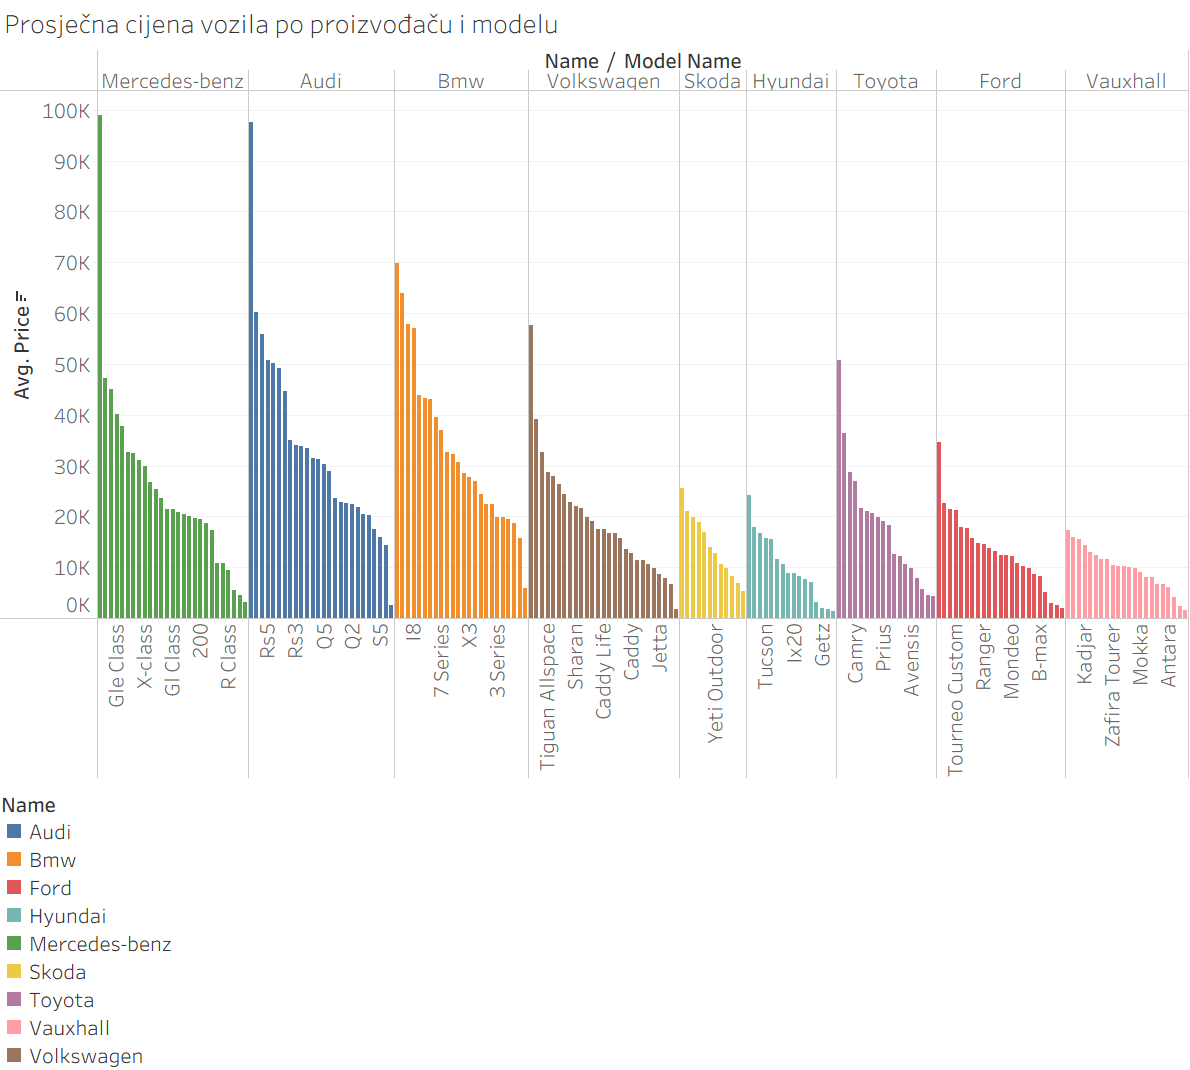
\includegraphics[width=0.9\textwidth]{slike/olap_analiza/8-prosječna-cijena-vozila-po-proizvođaču-i-modelu.png}
    \caption{Prosječna cijena vozila po proizvođaču i modelu}
    \label{fig:cijena-po-modelu}
\end{figure}

Stupčasti dijagram jasno demonstrira hijerarhiju vrijednosti kroz portfolije različitih proizvođača. Mercedes-Benz dominira premium segmentom s G Class modelom koji dostiže vrhunac od približno 100.000€, praćen S Class (~45.000€) i A Class (~40.000€) modelima, što potvrđuje strategiju vertikalnog pokrivanja luksuznog tržišta. Audi pokazuje najširi spektar cijena s flagship modelima (RS serija) koji dostižu 100.000€, demonstrirajući uspješnu premiumizaciju portfelja. BMW održava konzistentno visoke cijene kroz različite modele, potvrđujući pozicioniranje u upper-premium segmentu.

Volkswagen pokriva srednji do viši segment s modelima u rasponu 10.000-60.000€, što odražava strategiju "brand stretching" od mass-market prema premium pozicioniranju. Škoda iznenađuje s nekoliko modela u višem cjenovnom segmentu (~25.000€), što ukazuje na uspješnu evoluciju od budget prema value-premium brandiranju. Azijski proizvođači Toyota i Hyundai uglavnom se pozicioniraju u nižem do srednjem segmentu (5.000-25.000€), s Hyundai koji pokazuje jedan premium model, što signalizira pokušaje probijanja u više segmente. Ford i Vauxhall konzistentno zauzimaju najniži cjenovni segment (5.000-15.000€), potvrđujući focus na mass-market tržišnom segmentu.

\subsection{Analiza eksploatacijskih karakteristika}

Treća skupina analiza istražuje praktične aspekte korištenja vozila kroz kilometre, starost i potrošnju.

\subsubsection{Odnos starosti i kilometraže}

Scatter plot analiza otkriva obrazac korištenja vozila kroz vrijeme.

\begin{figure}[H]
    \centering
    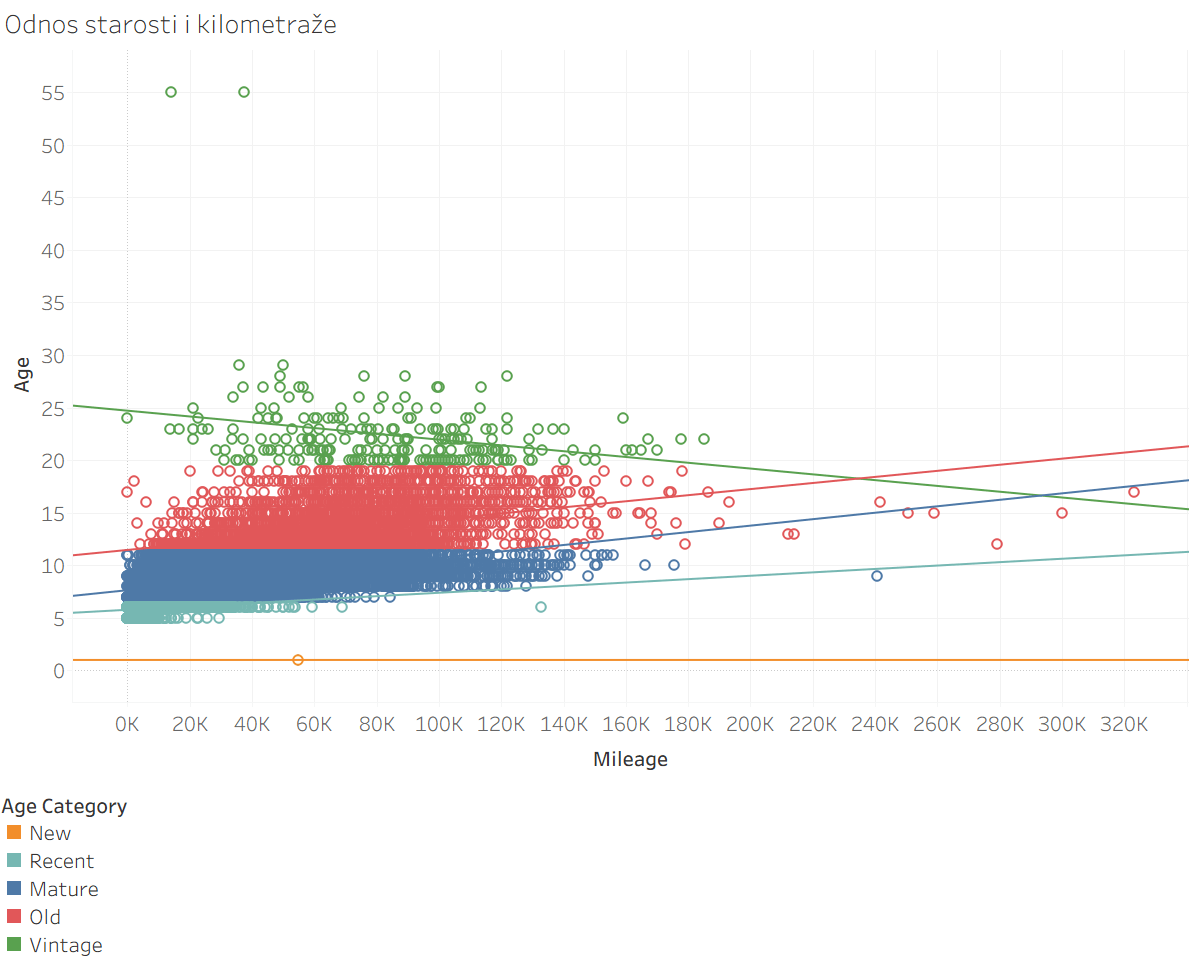
\includegraphics[width=0.9\textwidth]{slike/olap_analiza/9-odnos-starosti-i-kilometraže.png}
    \caption{Odnos starosti i kilometraže automobila}
    \label{fig:starost-kilometraza}
\end{figure}

Scatter plot vizualizacija s kategorizacijom vozila po starosti otkriva kompleksne obrasce korištenja kroz životni ciklus automobila. Vintage vozila (zelena, 20-55 godina starosti) pokazuju izuzetno varijabilnu kilometražu od minimalnih vrijednosti do preko 180.000 km, što odražava različite pristupe čuvanju - od garažnih kolekcijskih primjeraka do svakodnevno korištenih klasika.

Old vozila (crvena, 10-20 godina) demonstriraju najširu distribuciju kilometraže s jasnim trendom rasta, gdje većina vozila akumulira 50.000-140.000 km, što predstavlja tipičan obrazac deprecijacije kroz intenzivnu upotrebu. Mature vozila (plava, 5-15 godina) pokazuju umjerenu pozitivnu korelaciju s koncentracijom u rasponu 5.000-140.000 km, što ukazuje na stabilnu fazu korištenja.

Recent vozila (tirkizna, 2-8 godina) uglavnom se nalaze u rasponu do 80.000 km s linearnim trendom rasta, dok New vozila (narančasta, 0-5 godina) pokazuju najnižu kilometražu od oko 55.000 km (samo jedan primjerak). Trend linije po kategorijama otkrivaju da vintage vozila imaju najpoloženiji nagib (minimalno godišnje povećanje kilometraže), dok old i mature kategorije pokazuju najstrmiji rast, što potvrđuje intenzivnu upotrebu u srednjim i kasnim godinama životnog ciklusa vozila.

\subsubsection{Kilometraža po tipu motora}

Box plot analiza prikazuje distribuciju kilometraže prema tipovima motora.

\begin{figure}[H]
    \centering
    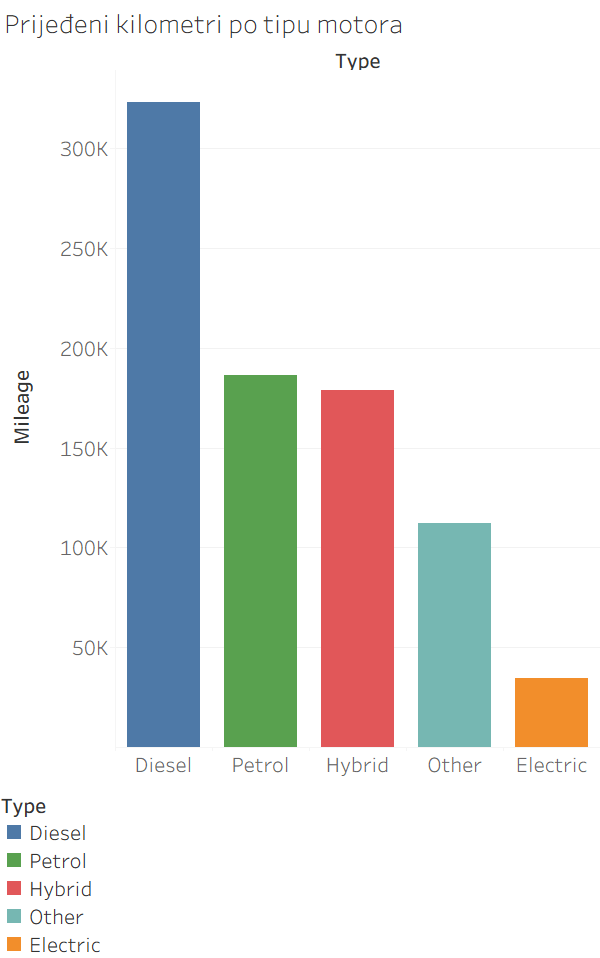
\includegraphics[width=0.7\textwidth]{slike/olap_analiza/10-prijeđeni-kilometri-po-tipu-motora.png}
    \caption{Prijeđeni kilometri po tipu motora}
    \label{fig:kilometri-tip-motora}
\end{figure}

Stupčasti dijagram jasno demonstrira značajne razlike u obrascima korištenja vozila prema tipovima motora. Dizelski motori dominiraju s prosječno 330.000 km, što potvrđuje njihovu primarnu ulogu u long-haul aplikacijama, komercijalnim vozilima i dugotrajnim putovanjima gdje ekonomičnost goriva postaje kritična. Benzinski motori zauzimaju drugo mjesto s 185.000 km, što odražava njihovu široku primjenu u svakodnevnoj urbano-suburbanoj mobilnosti.

Hibridni motori s prosječno 180.000 km pokazuju slične obrasce korištenja kao benzinski, što ukazuje na njihovu uspješnu integraciju u mainstream tržišni segment. Kategorija "Other" (uključujući LPG, CNG i alternativna goriva) s 115.000 km pozicionira se kao srednje-kilometražni segment, vjerojatno zbog specifičnih infrastrukturnih ograničenja i ciljanih aplikacija.

Električni motori pokazuju najnižu prosječnu kilometražu od samo 35.000 km, što odražava kombinaciju faktora: relativno recentnu adaptaciju tehnologije, ograničenja dosega, koncentraciju na urbano korištenje, te činjenicu da mnogi električni automobili još uvijek nisu prošli potpuni životni ciklus na tržištu rabljenih vozila.

\subsection{Tržišna analiza i trendovi}

Četvrta skupina analiza fokusira se na makroekonomske trendove i tržišne udjele.

\subsubsection{Udio proizvođača na tržištu}

Treemap vizualizacija kombinira tržišni udio s prosječnim cijenama proizvođača kroz veličinu i boju pravokutnika.

\begin{figure}[H]
    \centering
    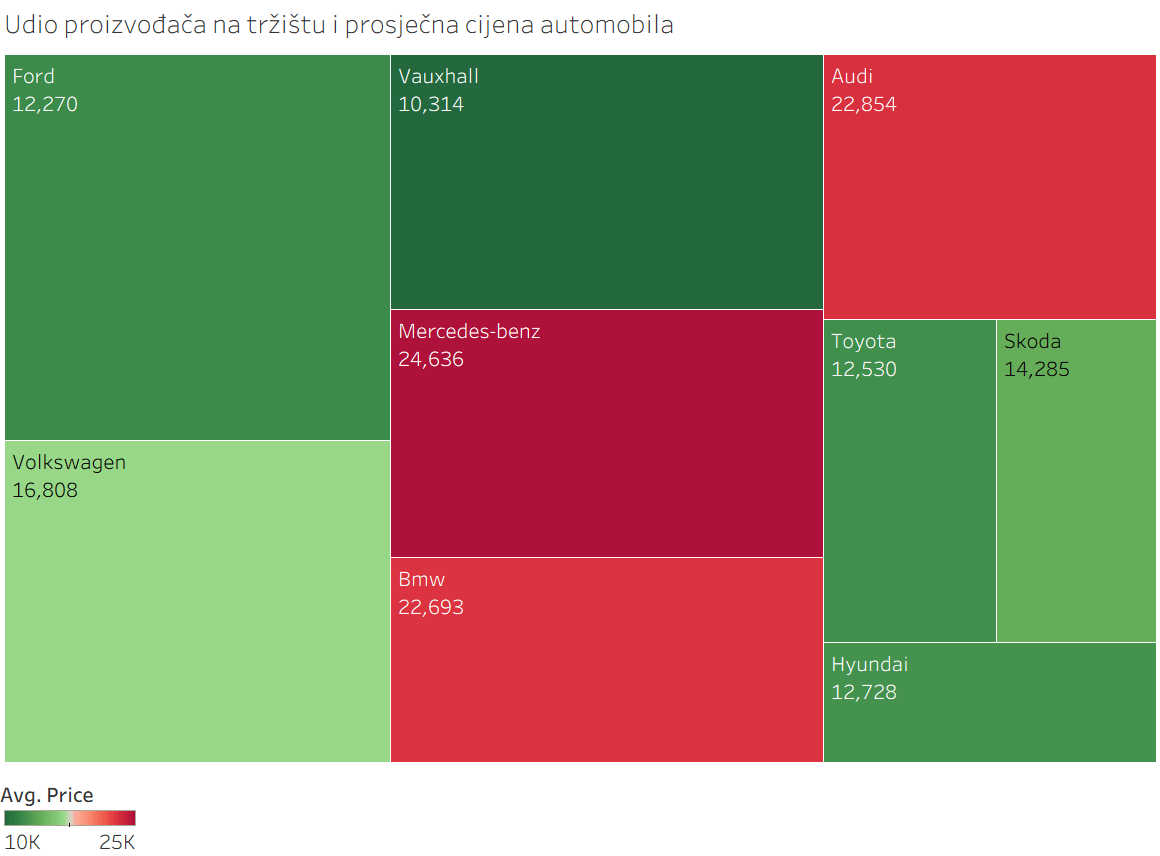
\includegraphics[width=0.9\textwidth]{slike/olap_analiza/11-udio-proizvođača-na-tržištu-i-prosječna-cijena-automobila.png}
    \caption{Udio proizvođača na tržištu i prosječna cijena automobila}
    \label{fig:udio-proizvođača}
\end{figure}

Treemap vizualizacija s preciznim podacima otkriva jasne obrasce između tržišnog volumena i cjenovnog pozicioniranja proizvođača automobila. Ford dominira apsolutnim tržišnim udjelom s 17.811 prodanih vozila pri prosječnoj cijeni od 12.270€, što naglašava klasičnu mass-market strategiju kroz visoki volumen i pristupačne cijene. Volkswagen zauzima drugo mjesto s 14.893 vozila i prosječnom cijenom od 16.808€, demonstrirajući uspješno balansiranje između volumena i umjereno višeg pozicioniranja.

Vauxhall s 13.258 vozila i najnižom prosječnom cijenom od 10.314€ pozicionira se kao budget opcija s značajnim tržišnim prisustvom. Njemačka premium trojka pokazuje inverzni obrazac: Mercedes-Benz (12.860 vozila, 24.636€), BMW (10.664 vozila, 22.693€) i Audi (10.565 vozila, 22.854€) postižu umjerene tržišne udjele ali najviše prosječne cijene, što potvrđuje strategiju premium pozicioniranja s fokusom na profitabilnost umjesto volumena.

Toyota (6.699 vozila, 12.530€), Škoda (6.188 vozila, 14.285€) i Hyundai (4.774 vozila, 12.728€) zauzimaju nižu polovinu tržišta s value-for-money pristupom, kombinirajući pristupačne cijene s umjerenim volumenima. Ova analiza ilustrira temeljnu dilemu automobilske industrije između strategije visokog volumena/niskih marži nasuprot niskog volumena/visokih marži.

\subsubsection{Geografska distribucija tipova mjenjača}

Stacked bar chart prikazuje preferencije tipova mjenjača po zemljama proizvođača kroz apsolutne brojeve vozila.

\begin{figure}[H]
    \centering
    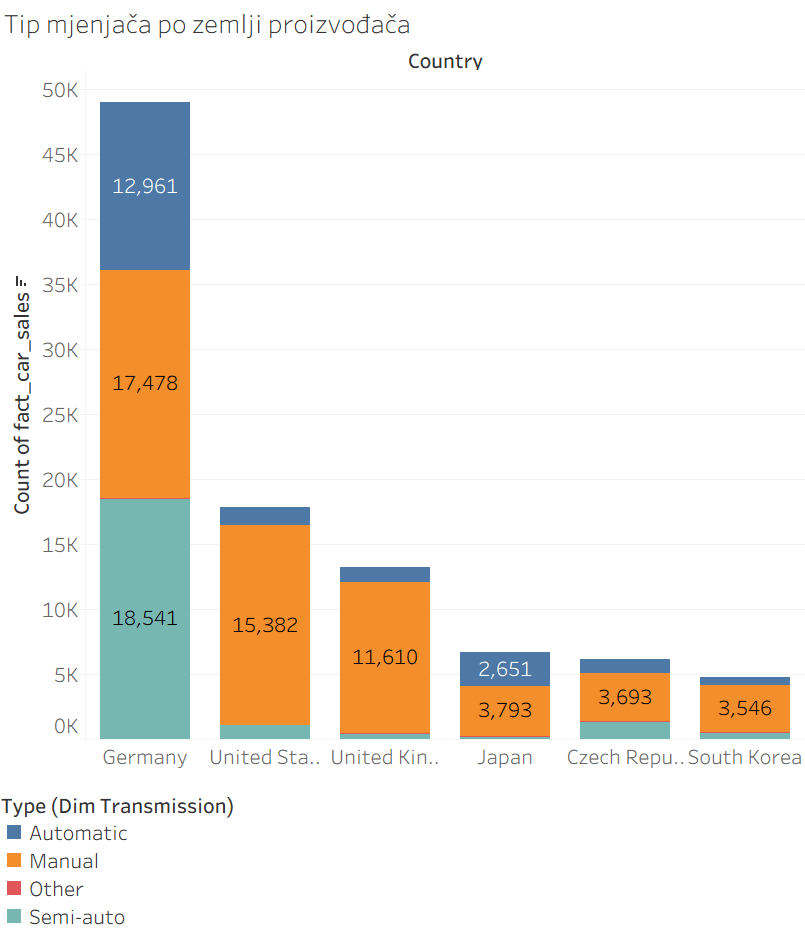
\includegraphics[width=0.9\textwidth]{slike/olap_analiza/12-tip-mjenjača-po-zemlji-proizvođača.png}
    \caption{Distribucija tipova mjenjača po zemlji proizvođača}
    \label{fig:mjenjac-zemlja}
\end{figure}

Stacked bar chart analiza otkriva karakteristike proizvodnje različitih zemalja zastupljenih na promatranom tržištu. Njemački proizvođači dominiraju ukupnim volumenom s približno 49.000 vozila, pri čemu ručni mjenjači čine značajan udio (17.478), praćeni semi-automatskim sustavima i automatskim mjenjačima. Ova distribucija odražava njemačku tradiciju inženjerske preciznosti u proizvodnji različitih tipova mjenjača.

Američki proizvođači (~18.000 vozila) i britanski proizvođači (~13.000 vozila) pokazuju sličan obrazac u proizvodnji s dominacijom ručnih mjenjača, što odražava prilagodbu ponude preferencama kupaca promatranog tržišta. Azijski proizvođači iz Japana (~6.000), Češke Republike (~6.000) i Južne Koreje (~5.000) također se fokusiraju na ručne mjenjače, ali s većim udjelom automatskih sustava što ukazuje na njihovu proizvodnu specijalizaciju i tehnološku orijentaciju.

Zanimljivo je prisustvo semi-automatskih mjenjača prvenstveno u njemačkoj proizvodnji, što odražava inovativni pristup kombiniranja prednosti oba tipa mjenjača. Ovo je tipično za njemačke premium proizvođače koji nastoje ponuditi optimum između performansi i udobnosti.

\subsection{Distribucijska analiza}

Peta skupina fokusira se na statističke distribucije ključnih varijabli.

\subsubsection{Distribucija cijena}

Histogram distribucije automobila po cijenama otkriva dominantne tržišne segmente.
\begin{figure}[H]
    \centering
    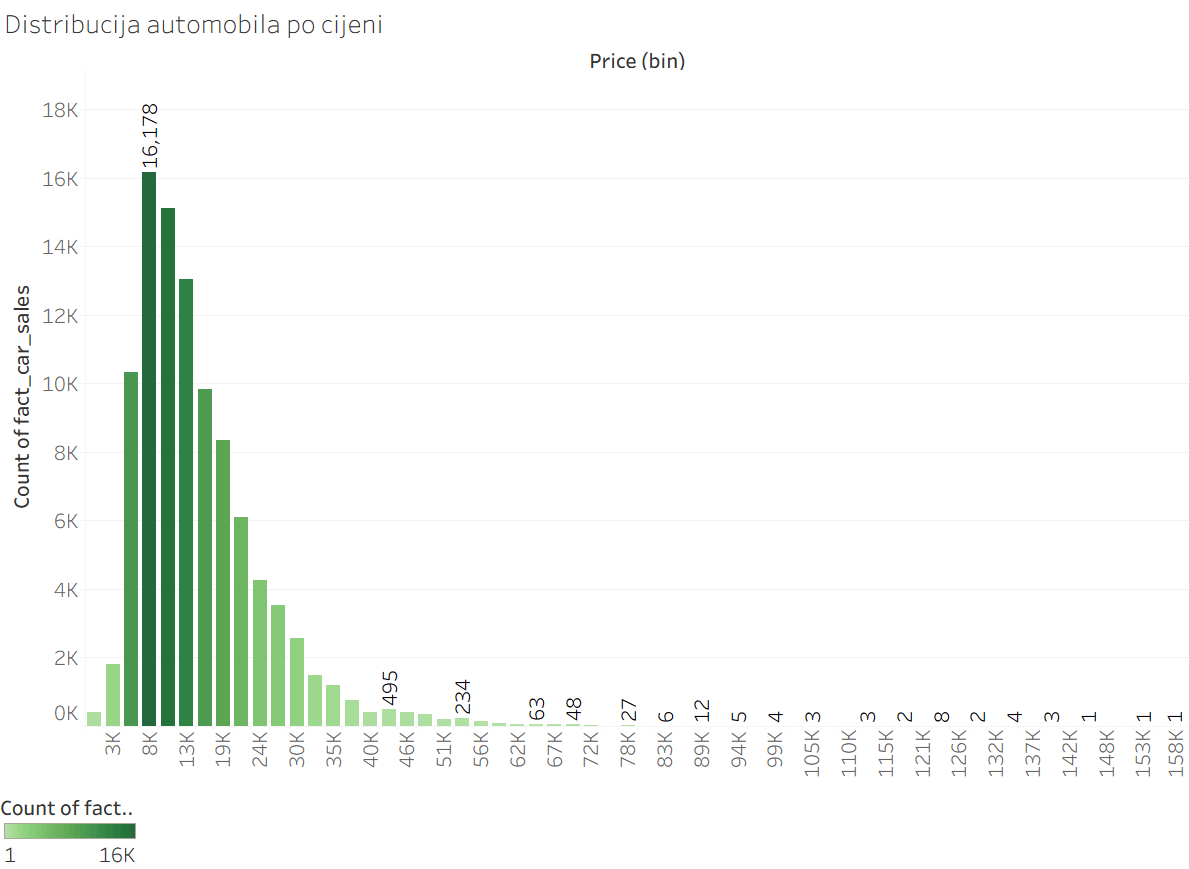
\includegraphics[width=0.9\textwidth]{slike/olap_analiza/13-distribucija-automobila-po-cijeni.png}
    \caption{Distribucija automobila po cijeni}
    \label{fig:distribucija-cijena}
\end{figure}

Histogram jasno demonstrira izrazito desno-skrenutu (right-skewed) distribuciju s dominantnim vrhom u najnižem cjenovnom segmentu. Najveća koncentracija vozila (16.178) nalazi se u rasponu 8-13 tisuća eura, što potvrđuje dominaciju budget segmenta na promatranom tržištu. Distribucija pokazuje kontinuirani pad broja vozila s porastom cijene.

Karakteristična je pojava "dugog repa" koji se proteže do najskupljih segmenata (140k-160k€) s minimalnim brojem vozila (1-8 primjeraka), što reprezentira ekskluzivni luxury segment. Ova distribucija tipična je za sekundarna tržišta automobila gdje dominiraju rabljena vozila u pristupačnim cjenovnim kategorijama, s postupnim smanjenjem zastupljenosti prema premium i luxury segmentima.

\subsubsection{Distribucija kilometraže}

Slična analiza za kilometražu otkriva obrasce korištenja vozila.

\begin{figure}[H]
    \centering
    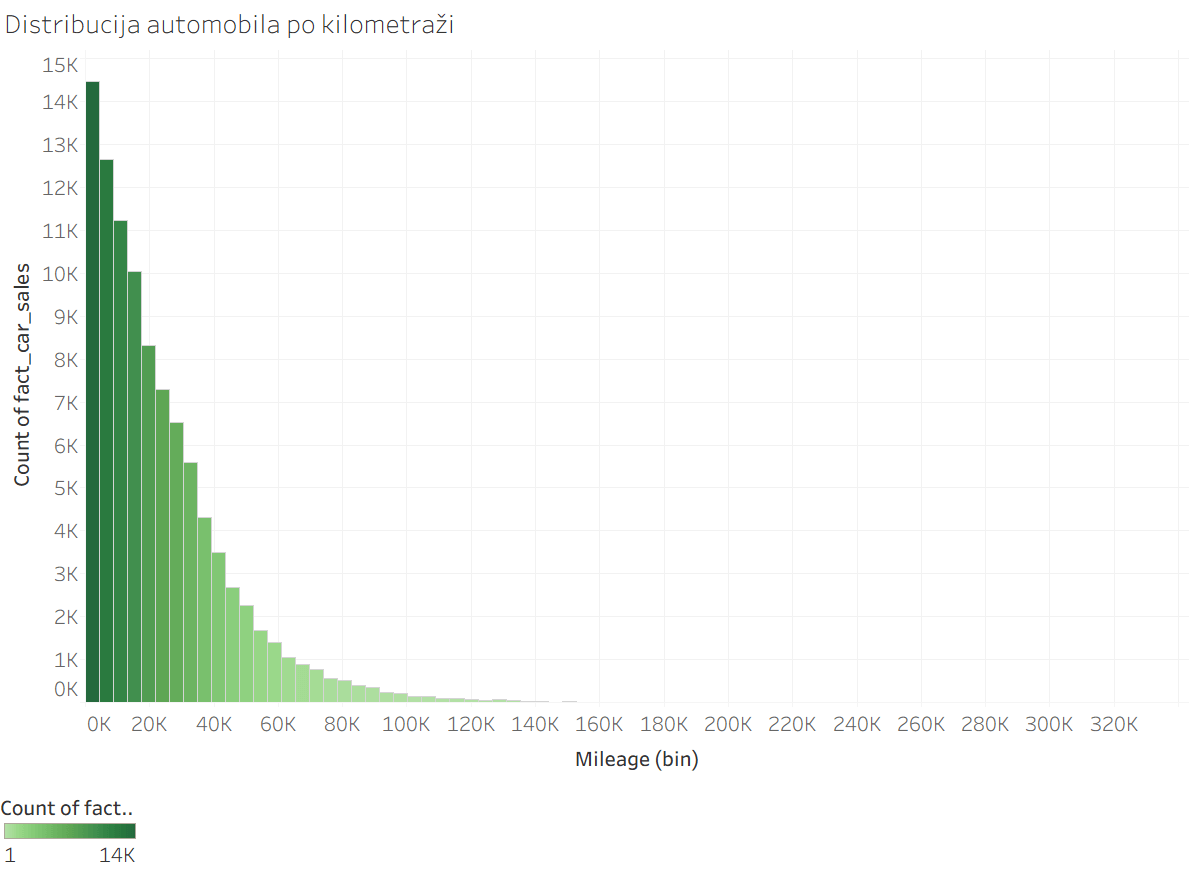
\includegraphics[width=0.9\textwidth]{slike/olap_analiza/14-distribucija-automobila-po-kilometraži.png}
    \caption{Distribucija automobila po kilometraži}
    \label{fig:distribucija-kilometraza}
\end{figure}

Histogram otkriva izrazito desno-skrenutu distribuciju s dominantnim vrhom u segmentu najniže kilometraže. Najveća koncentracija vozila (preko 14.000) nalazi se u rasponu 0-20.000 km, što ukazuje na značajan udio vozila s minimalnim korištenjem - vjerojatno nova ili rijetko rabljena vozila.

Distribucija pokazuje strm eksponencijalni pad s povećanjem kilometraže: od drugog vrha s približno 12.500 vozila u rasponu 20-40k km, frekvencija kontinuirano opada kroz srednje segmente (10-8k vozila u rasponu 40-80k km), sve do visokih kilometraža gdje se nalazi svega nekoliko stotina vozila.

Karakteristična je pojava "dugog repa" koji se proteže do ekstremnih kilometraža (preko 300.000 km) s minimalnim brojem vozila, što predstavlja komercijalna vozila ili intenzivno korištene automobile. Ova distribucija tipična je za tržišta koja kombiniraju nova/demonstration vozila s rabljenim vozilima različitih stupnjeva korištenja, pri čemu dominiraju vozila s niskim do umjerenim kilometražama.

\subsubsection{Usporedba distribucije po tipu prijenosa}

Box plot omogućuje detaljnu usporedbu distribucije cijena prema tipovima mjenjača.

\begin{figure}[H]
    \centering
    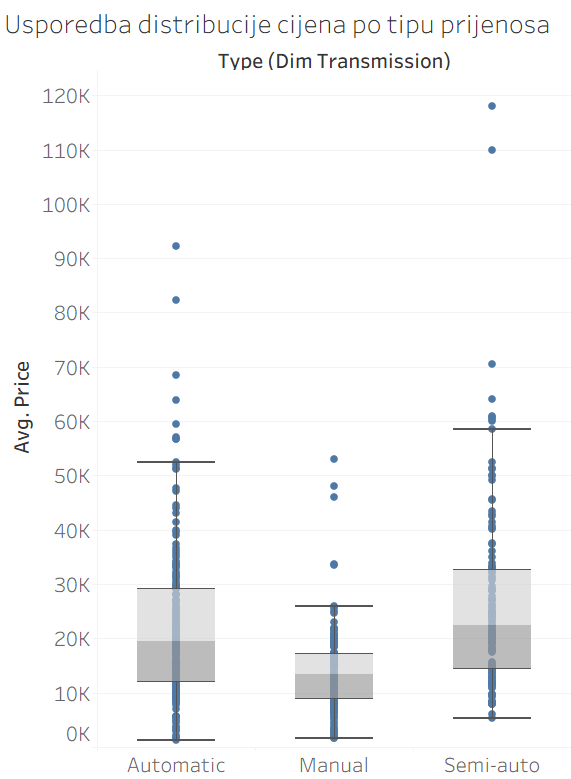
\includegraphics[width=0.9\textwidth]{slike/olap_analiza/15-usporedba-distribucije-cijena-po-tipu-prijenosa.png}
    \caption{Usporedba distribucije cijena po tipu prijenosa}
    \label{fig:distribucija-prijenos}
\end{figure}

Box plot analiza otkriva značajne razlike u cjenovnim distribucijama između tipova mjenjača. Ručni mjenjači pokazuju najnižu cjenovnu distribuciju s medijanom oko 15.000€ i kompaktnim interkvartilnim rasponom (10.000-20.000€), što potvrđuje njihovu dominaciju u budget i mainstream segmentima tržišta. Nekoliko outliera dostiže do 53.000€, predstavljajući premium sportske modele s ručnim mjenjačima.

Automatski mjenjači zauzimaju srednji segment s medijanom oko 20.000€ i širim interkvartilnim rasponom (13.000-30.000€). Značajan broj outliera proteže se do ekstremnih vrijednosti preko 90.000€, što ukazuje na prisutnost automatskih mjenjača kroz sve tržišne segmente - od mainstream do luxury vozila.

Semi-automatski mjenjači dominiraju najvišim cjenovnim pozicioniranjem s medijanom oko 22.000€ i širim interkvartilnim rasponom (15.000-32.000€). Outlieri dosežu do 120.000€, što potvrđuje prisutnost ovog tipa mjenjača u premium i luxury segmentima, osobito kod njemačkih proizvođača koji kombiniraju sportske performanse s naprednom automatizacijom.

\subsection{Analiza efikasnosti i performansi}

Šesta skupina istražuje tehničke performanse i efikasnost vozila.

\subsubsection{Potrošnja goriva prema starosti}

Stupčasti dijagram prikazuje kako se mijenja efikasnost vozila s godinama starosti.

\begin{figure}[H]
    \centering
    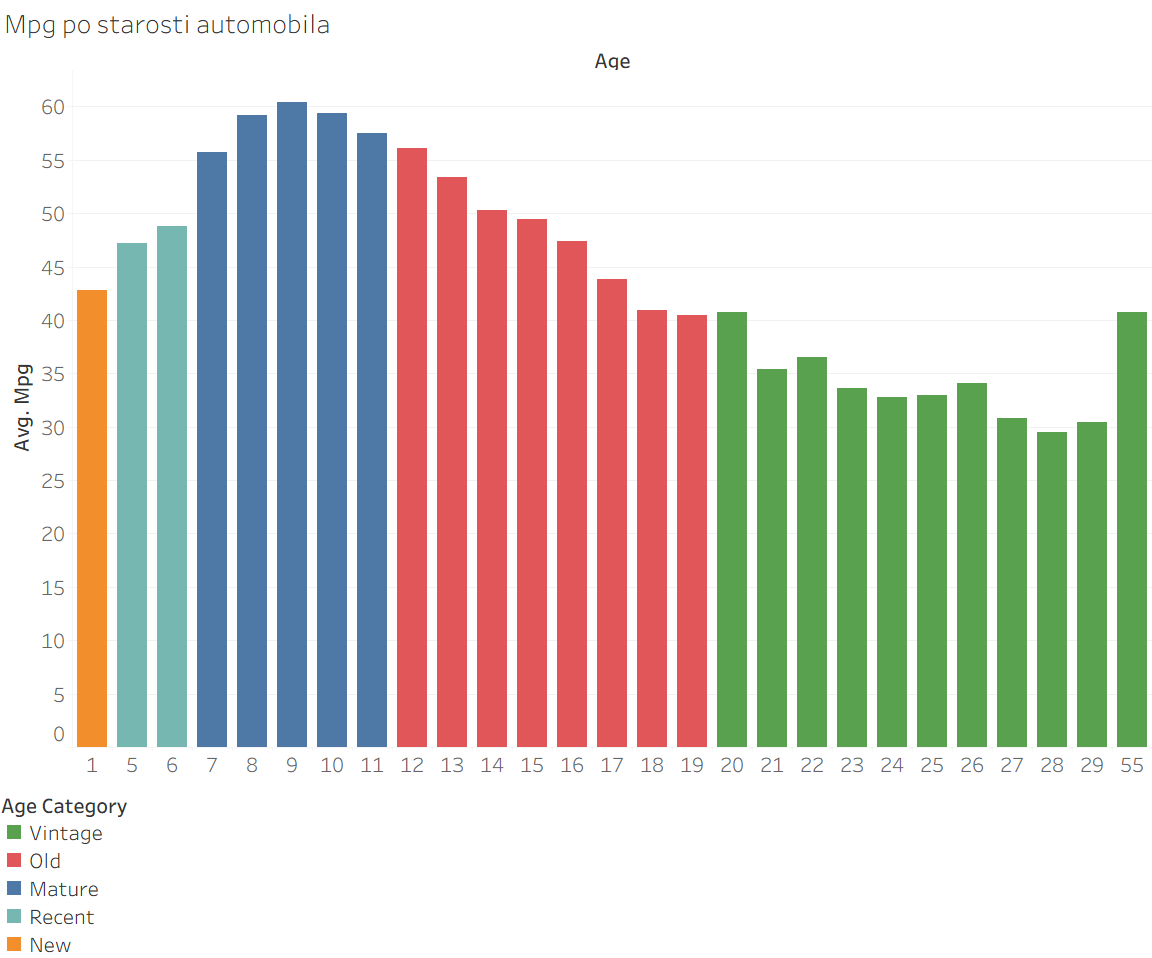
\includegraphics[width=0.9\textwidth]{slike/olap_analiza/16-mpg-po-starosti-automobila.png}
    \caption{Milja po galonu (MPG) prema starosti automobila}
    \label{fig:mpg-starost}
\end{figure}

Analiza otkriva kompleksan obrazac efikasnosti goriva kroz različite generacije vozila s jasno izraženim kategorijskim trendovima. Najstarija vozila (New - 1-5 godina) postižu umjerenu efikasnost, što odražava suvremene tehnološke standarde ali s prostorem za poboljšanje.

Skok u efikasnosti vidljiv je u kategoriji Recent vozila (5-7 godina) koja dosežu vrhunac od 49 MPG, što predstavlja optimum između tehnološke zrelosti i regulatornih zahtjeva tog razdoblja. Mature vozila (7-12 godina) održavaju visoku efikasnost od 57-60 MPG, potvrđujući da je to razdoblje predstavljalo zlatno doba fuel-efficient tehnologija.

Starija vozila pokazuju postupan pad efikasnosti: Old kategorija (12-20 godina) varira između 41-56 MPG, dok Vintage vozila (preko 20 godina) pokazuju najnižu i najvarijabilniju efikasnost (31-41 MPG). Zanimljiv je skok na 55. godini starosti, što vjerojatno predstavlja oldtimer vozila s posebno održavanim motorima.

Ovaj trend sugerira da su vozila iz 2010-ih godina bila optimalno dizajnirana za fuel efficiency, prije nego što su novi tehnološki zahtjevi (hibridizacija, elektrifikacija) privremeno snizili prosječnu efikasnost konvencionalnih motora u najnovijim vozilima.

\subsection{Fiskalna analiza}

Sedma skupina analiza istražuje porezne aspekte i njihovu povezanost s karakteristikama vozila.

\subsubsection{Odnos cijene i poreza po regijama}

Scatter plot s trend linijama prikazuje korelaciju između cijene vozila i godišnjeg poreza po trima regijama: Aziji, Europi i Sjevernoj Americi.

\begin{figure}[H]
    \centering
    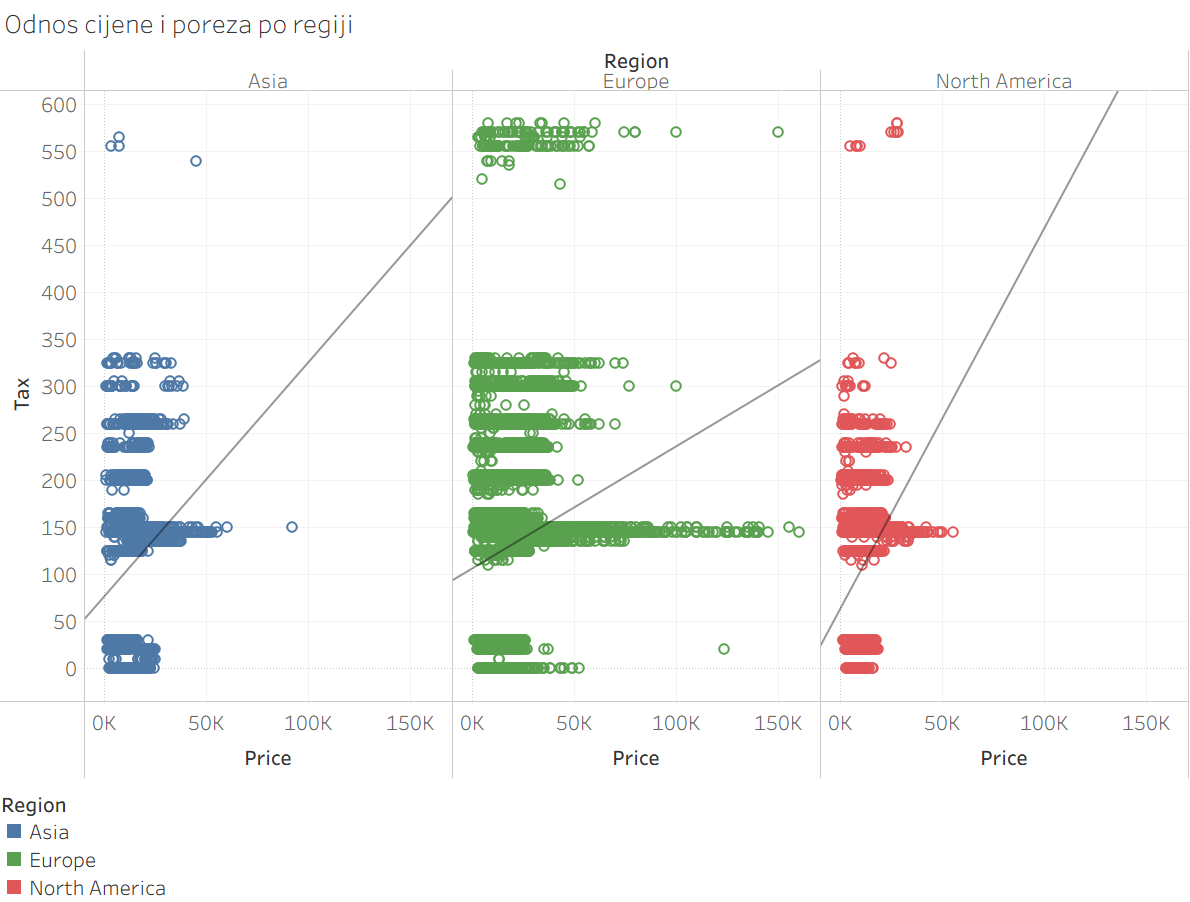
\includegraphics[width=0.9\textwidth]{slike/olap_analiza/17-odnos-cijene-i-poreza-po-regiji.png}
    \caption{Odnos cijene i poreza po regijama}
    \label{fig:cijena-porez-regija}
\end{figure}

Analiza otkriva značajne razlike u poreznim strukturama među regijama. Sjeverna Amerika pokazuje najstrmiju trend liniju, što ukazuje na najagresivniji progresivni porezni sustav gdje porez značajno raste s cijenom vozila. Azijska tržišta pokazuju umjerenu korelaciju s koncentracijom vozila u nižem cjenovnom segmentu (do €50.000), dok Europa ima najblažu trend liniju unatoč tome što pokriva srednji i viši cjenovni segment. Trend linije jasno prikazuju da Sjeverna Amerika primjenjuje najstroži progresivni porezni sustav, dok Europa ima najmanje izraženu progresivnost poreza u odnosu na cijenu vozila.

\subsubsection{Porez kao postotak cijene}

Calculated field analiza prikazuje porezno opterećenje kao postotak vrijednosti vozila kroz heatmapu koja kombinira proizvođače i tipove motora.

\begin{figure}[H]
    \centering
    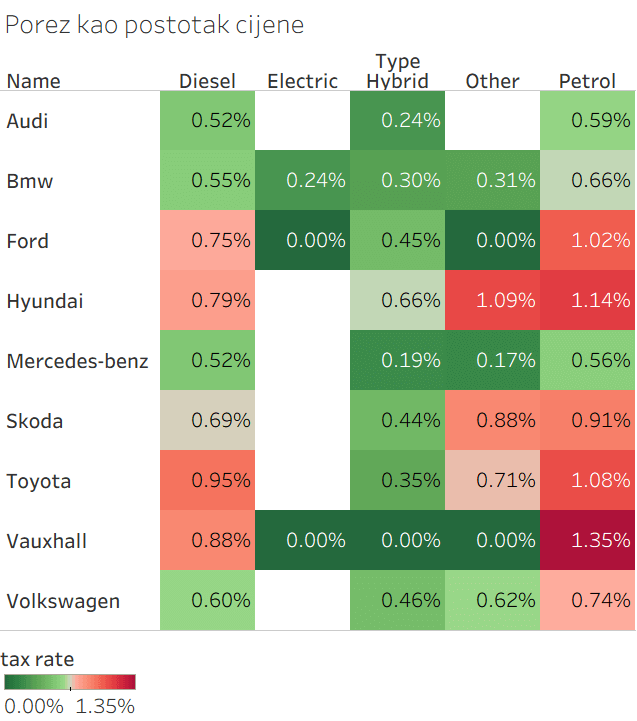
\includegraphics[width=0.9\textwidth]{slike/olap_analiza/18-porez-kao-postotak-cijene.png}
    \caption{Porez kao postotak cijene vozila}
    \label{fig:porez-postotak}
\end{figure}

Heatmap analiza otkriva kompleksne obrasce poreznog opterećenja koji se kreću u rasponu od 0,00\% do 1,35\% vrijednosti vozila. Najviše porezno opterećenje snose Vauxhall, Toyota i Hyundai vozila na benzin. Ovo ukazuje na to da se mass-market brendovi suočavaju s relativno višim poreznim teretom u odnosu na vrijednost vozila.

Premium njemački proizvođači pokazuju umjereniji porezni teret, što sugerira da porezni sustav favorizira skuplja vozila kroz niže relativne stope. Električni, hibridni i drugi tipovi motora pokazuju nulte ili vrlo niske stope poreza, što vjerojatno odražava porezne poticaje za ekološki prihvatljive tehnologije. Najveća porezna opterećenja nalazimo kod benzinaca i dizelaša, čime se vjerojatno želi potaknuti prelazak na čišće tehnologije.

\subsubsection{Prosječni porez po zemljama proizvođača}

Bar chart rangira zemlje prema prosječnom godišnjem porezu na vozila, otkrivajući varijacije u nacionalnim poreznim politikama.

\begin{figure}[H]
    \centering
    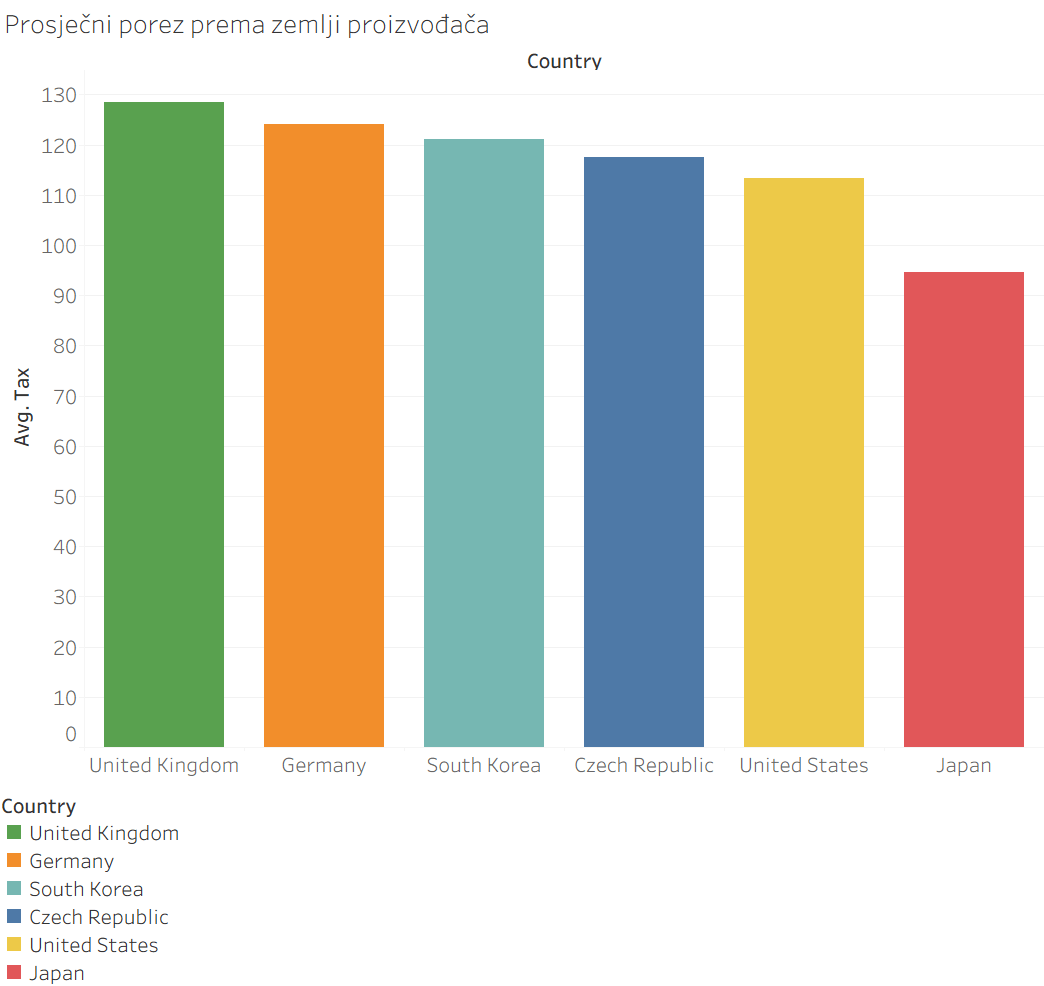
\includegraphics[width=0.9\textwidth]{slike/olap_analiza/19-prosječni-porez-prema-zemlji-proizvođača.png}
    \caption{Prosječni porez prema zemlji proizvođača}
    \label{fig:porez-zemlja}
\end{figure}

Analiza otkriva jasnu hijerarhiju poreznih opterećenja prema zemljama porijekla proizvođača na promatranom tržištu. Vozila britanskih proizvođača nose najviši prosječni porezni teret od 128€, praćena njemačkim proizvođačima s 125€. Ova razlika može odražavati diferencirane porezne stope koje lokalni porezni sustav primjenjuje na vozila različitog porijekla.

Vozila južnokorejskih (121€) i čeških proizvođača (118€) opterećena su umjerenim poreznim stopama, dok američki proizvođači uživaju nešto povoljniji tretman s prosječnim porezom od 114€. Japanski proizvođači imaju najniži prosječni porezni teret od 96€, što može ukazivati na preferencijalnu poreznu politiku prema vozilima iz te zemlje.

Ove varijacije u poreznom opterećenju prema zemlji porijekla proizvođača stvaraju različite konkurentne pozicije na tržištu, gdje vozila japanskih proizvođača uživaju poreznu prednost koja može utjecati na njihovu cjenovnu konkurentnost i tržišni udio.

\subsection{Kombinirana analiza dimenzija}

Završna analiza kombinira dimenzije za sveobuhvatan uvid u tržišne dinamike.

\subsubsection{Multi-dimenzijska analiza starosti}

Kombinirana analiza poreza i kilometraže prema kategorijama starosti vozila.

\begin{figure}[H]
    \centering
    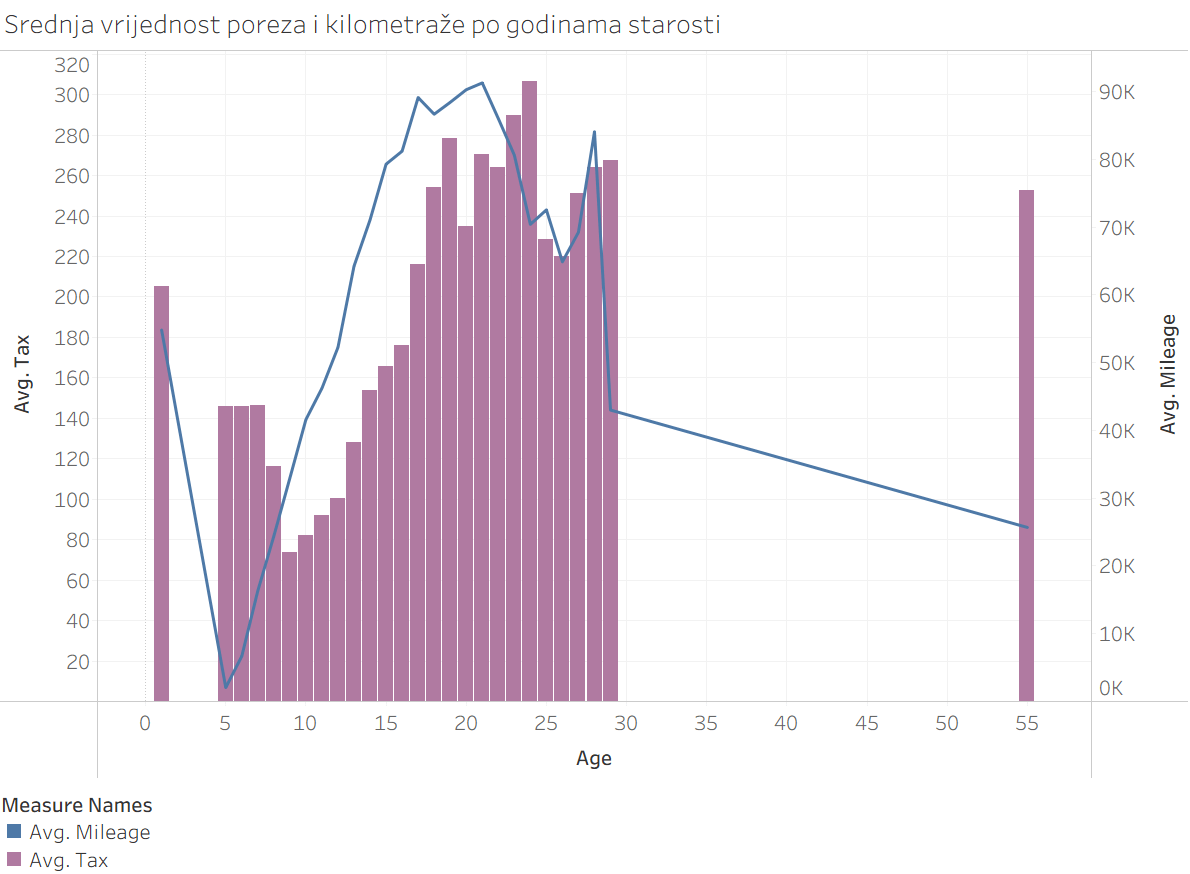
\includegraphics[width=0.9\textwidth]{slike/olap_analiza/20-srednja-vrijednost-poreza-i-kilometraže-po-godinama-starosti.png}
    \caption{Srednja vrijednost poreza i kilometraže po godinama starosti}
    \label{fig:kombinirana-analiza}
\end{figure}

Kombinirana vizualizacija otkriva fascinantan inverzni odnos između starosti vozila, poreza i kilometraže kroz životni ciklus automobila. Analiza demonstrira kako se ove tri ključne dimenzije međusobno utječu kroz različite faze korištenja vozila.

\textbf{Faza novijih vozila (0-15 godina):} Vozila u ovoj kategoriji pokazuju relativno nizak prosječni porez (50-200€ godišnje) uz umjerenu kilometražu (20.000-40.000 km). Ova faza karakterizirana je početnim razdobljem korištenja gdje vozila još uvijek zadržavaju visoku vrijednost i relativno nisko porezno opterećenje.

\textbf{Faza zrelih vozila (15-25 godina):} Uočava se dramatičan porast prosječnog poreza koji dostiže vrhunac oko 310€ u 24. godini starosti, dok kilometraža postupno raste prema 90.000 km. Ovaj fenomen ukazuje na to da starija vozila, unatoč manjoj tržišnoj vrijednosti, mogu nositi veći porezni teret - vjerojatno zbog poreznih politika koje penaliziraju starije, manje ekološki prihvatljive motore.

\textbf{Faza vintage vozila (25+ godina):} Nakon 25. godine starosti uočava se nagao pad prosječnog poreza (s 310€ na oko 80€), što sugerira postojanje poreznih olakšica za oldtimer vozila. Kilometraža u ovoj fazi pokazuje veliku varijabilnost, od minimalnih vrijednosti kod kolekcijskih vozila do preko 180.000 km kod aktivno korištenih klasika.

Graf nam otkriva da porast poreza generalno prati povećanje kilometraže koje raste s godinama starosti, s izuzetkom vintage vozila kod kojih kilometraža ne prati visoke porezne stope. Ovo se može objasniti time da su neka od vintage vozila bila aktivno vožena tijekom godina, dok su druga očuvana kao kolekcionarski primjerci s minimalnom upotrebom.

Na ovom grafu demonstrirane su napredne OLAP mogućnosti kroz kombiniranje više mjera i dimenzija, omogućujući holistički pogled na životni ciklus vozila i pružajući vrijedne uvide za optimizaciju poreznih politika, procjenu vrijednosti vozila i razumijevanje obrazaca korištenja kroz različite generacije automobila.